\documentclass[]{article}
\usepackage[top=1.5in,bottom=1.5in,left=1in,right=1in]{geometry}
\usepackage{tikz}
\usetikzlibrary{shapes.geometric}
\usepackage{subcaption}
\usepackage{xcolor}
\usepackage[colorlinks,allcolors=blue]{hyperref}
\usepackage[noabbrev]{cleveref}


\title{
    {\LARGE Rules for the Game of}
    \\[1ex]
    {\Huge\bf Chexers}
}
\author{
    \textbf{Matthew Farrugia-Roberts}
    \\
    \textit{The University of Melbourne}
    \\
    \href
      {mailto:matt.farrugia@unimelb.edu.au}
      {\tt matt.farrugia@unimelb.edu.au}
}
\date{2019}


% Custom TikZ commands
\newcommand{\piece}[4] {
    \node[draw,circle,minimum size=6.8mm,fill=white] at ({#1}, {#2}) {};
    \node[draw,circle,minimum size=5.8mm,very thick,{#3}] at ({#1}, {#2}) {};
    \node[] at ({#1}, {#2}) {${#4}$};
}
\newcommand{\hex}[4] {
    \node[hex,fill={#3}] at ({#1}, {#2}) {};
    \node[hex,thick,draw={#3},fill={#3!10}] at ({#1}, {#2}) {};
    \node at ({#1}, {#2}) {{#4}};
}
\newcommand{\board} {
    \tikzset{
        hex/.style={
            regular polygon,
            regular polygon sides=6,
            minimum size=10mm,
            inner sep=0mm,
            outer sep=0mm,
            rotate=30,
            draw
        },
        x={(4.33mm,7.5mm)},
        y={(8.66mm,0mm)}
    }
    \foreach \r/\q in {
                 +3/-3,+3/-2,+3/-1,+3/+0,
              +2/-3,+2/-2,+2/-1,+2/+0,+2/+1,
           +1/-3,+1/-2,+1/-1,+1/+0,+1/+1,+1/+2,
        +0/-3,+0/-2,+0/-1,+0/+0,+0/+1,+0/+2,+0/+3,
           -1/-2,-1/-1,-1/+0,-1/+1,-1/+2,-1/+3,
              -2/-1,-2/+0,-2/+1,-2/+2,-2/+3,
                 -3/+0,-3/+1,-3/+2,-3/+3,
    }
        \node[hex,fill=black!5] at (\r, \q) {};
}

\begin{document}


\maketitle

\vfill

\begin{quote}
\emph{Chexers} is a three-player hexagonal turn-based race game. Test
the loyalty of your band of two-faced checkerpieces as you charge them
through a twisting and treacherous battleground. Will all your pieces
stay true to your cause? Can you earn yourself some new followers in the
chaos? To win this tumultuous chase, you must double-cross and
triple-cross your way across the finish line before your
opponents---three, two, one\ldots{} go!
\end{quote}

\vfill

\section*{Setup}

\emph{Chexers} plays on a hexagonal \textbf{board} of 37 \textbf{hexes},
as illustrated in \Cref{fig:board}.
%
Three \textbf{players} (\textbf{Red}, \textbf{Green}, and \textbf{Blue})
play the game.
Each player initially controls 4 \textbf{pieces} of their \textbf{colour}.
The pieces begin in the configuration shown below in \Cref{fig:board},
\textbf{occupying} hexes along three edges of the board.

\begin{figure}[ht!]
    \centering
    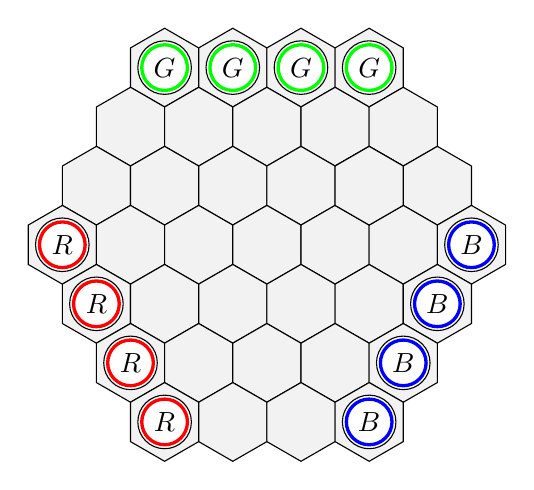
\begin{tikzpicture}
        \board
        \piece{-3}{+0}{red}{R}
        \piece{-2}{-1}{red}{R}
        \piece{-1}{-2}{red}{R}
        \piece{+0}{-3}{red}{R}
        \piece{+3}{-3}{green}{G}
        \piece{+3}{-2}{green}{G}
        \piece{+3}{-1}{green}{G}
        \piece{+3}{+0}{green}{G}
        \piece{-3}{+3}{blue}{B}
        \piece{-2}{+3}{blue}{B}
        \piece{-1}{+3}{blue}{B}
        \piece{+0}{+3}{blue}{B}
    \end{tikzpicture}
    \caption{
    \label{fig:board}
        Board with 37 hexes and starting configuration of 12 pieces:
        4~Red ($R$), 4~Green ($G$), 4~Blue ($B$).
    }
\end{figure}

\vfill

\newpage

\section*{Gameplay}

Players take turns, starting with Red, followed by Green, followed by
Blue. This cycle repeats until the game ends. On each turn, the current
player must take a single \textbf{action} involving a piece in their
colour, if possible. This action may be a \textbf{move action}, a
\textbf{jump action}, or an \textbf{exit action}.
%
If no such actions are possible the player must \textbf{pass} instead,
taking no action. A player cannot pass if they have available actions
(for example, a player can only pass if they have no remaining pieces or
their remaining pieces are all `blocked' by other pieces).
Each type of action is described in the following sections.

\subsection*{Move actions}

A \textbf{move action} (a `move') involves moving a piece from the hex
it currently \textbf{occupies} to an \textbf{adjacent} hex (one of the
at-most-six hexes in direct contact with the current hex on the board).
For the move action to take place, the adjacent hex must not be occupied
by another piece. A configuration illustrating available move actions is
shown in \Cref{fig:move}.

\subsection*{Jump actions}

A \textbf{jump action} (a `jump') involves moving a piece from its
current hex to an unoccupied hex \textbf{opposite} some occupied
adjacent hex. That is, a piece `jumps over' an adjacent piece onto the
hex directly on the other side from where it started. \Cref{fig:jump}
explores an example configuration to illustrate these concepts.

The adjacent piece (the one to be `jumped over') may have any colour. If
this piece is a different colour from the jumping piece, then it will be
\textbf{converted}---its colour will change to the colour of the jumping
piece as a result of the jump action. In this way, jump actions enable a
player to `gain control' of additional pieces.

\begin{figure}[ht!]
\centering
\begin{subfigure}{.35\textwidth}
    \centering
    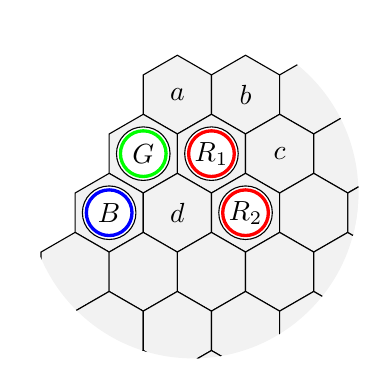
\begin{tikzpicture}
        \clip (-1.1,+1.0)  circle (2.1);
        \board
        \piece{+1}{-3}{blue}{B}
        \piece{+2}{-3}{green}{G}
        \piece{+2}{-2}{red}{R_1}
        \piece{+1}{-1}{red}{R_2}
        \node at (+3,-3) {$a$};
        \node at (+3,-2) {$b$};
        \node at (+2,-1) {$c$};
        \node at (+1,-2) {$d$};
    \end{tikzpicture}
    \caption{\label{fig:move}
        % \textbf{Move actions:}
        In this configuration, the piece $R_1$ has an available
        \textbf{move action} to each of the hexes marked $a$, $b$, $c$
        and $d$. Though the hexes occupied by $G$ and $R_2$ are also
        adjacent, moves to these hexes are not available since they are
        occupied. $G$ is on a hex near an edge of the board and has only 4
        adjacent hexes to begin with; since 2 of them are occupied (by $B$
        and $R_1$), $G$ can only move to hex $a$ or hex $d$.
    }
\end{subfigure}
\begin{subfigure}{.01\textwidth}
\phantom{SP}
\end{subfigure}
\begin{subfigure}{.62\textwidth}
    \centering
    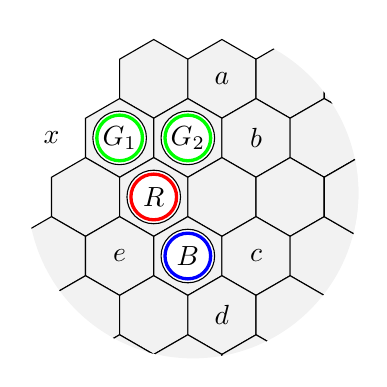
\begin{tikzpicture}
        \clip (-0.8,+0.8)  circle (2.1);
        \board
        \piece{+2}{-3}{green}{G_1}
        \piece{+2}{-2}{green}{G_2}
        \piece{+1}{-2}{red}{R}
        \piece{+0}{-1}{blue}{B}
        \node at (+3,-2) {$a$};
        \node at (+2,-1) {$b$};
        \node at (+0,+0) {$c$};
        \node at (-1,+0) {$d$};
        \node at (+0,-2) {$e$};
        \node at (+2,-4) {$x$};
    \end{tikzpicture}
    \caption{\label{fig:jump}
        % \textbf{Jump actions:}
        In this configuration, $G_1$ has a \textbf{jump action} available
        over $G_2$ to the horizontally opposite hex marked $b$.
        $G_1$ cannot jump over $R$ because the hex opposite $R$
        is occupied (by $B$). Note that $G_1$ cannot jump all the way to
        the hex marked $d$ either: a jumping piece may only go over a single
        hex. $G_2$ can jump over $R$ because the opposite hex from
        $G_2$'s perspective, $e$, is unoccupied
        (\emph{this jump action will result in the \textbf{conversion}
        of $R$ to a Green piece}).
        $G_2$ cannot jump over $G_1$ because there is no hex opposite $G_1$
        from $G_2$'s perspective
        (such a hex would have to be at the position marked $x$).
        Note further that `jump sequences' are not allowed:
        $G_2$ cannot jump over $R$ to $e$ and then over $B$ to $c$
        in one action, for example.
    }
\end{subfigure}
\caption{\label{fig:movejump}
    These partial board configurations exemplify the rules for
    move actions and jump actions.
}
\end{figure}

\subsection*{Exit actions}

An \textbf{exit action} (an `exit') involves a piece `leaving the
board'. These actions are only possible when a piece occupies some hex
on the edge of the board directly opposite the edge where the
controlling player's pieces started the game (as per \Cref{fig:board}) The
exiting piece is removed from the board (leaving its hex unoccupied).
\Cref{fig:exit} outlines the hexes that allow exit actions for each player,
and shows some examples of available exit actions.

\begin{figure}[ht!]
\centering
\begin{subfigure}{.35\textwidth}
    \centering
    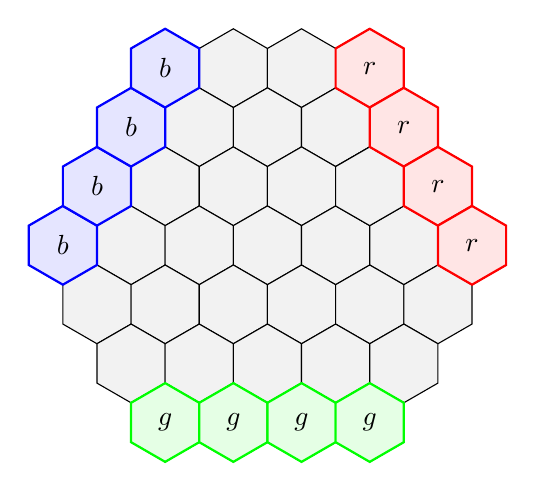
\begin{tikzpicture}
        \board
        \hex{+3}{+0}{red}{$r$}
        \hex{+2}{+1}{red}{$r$}
        \hex{+1}{+2}{red}{$r$}
        \hex{+0}{+3}{red}{$r$}
        \hex{-3}{+0}{green}{$g$}
        \hex{-3}{+1}{green}{$g$}
        \hex{-3}{+2}{green}{$g$}
        \hex{-3}{+3}{green}{$g$}
        \hex{+0}{-3}{blue}{$b$}
        \hex{+1}{-3}{blue}{$b$}
        \hex{+2}{-3}{blue}{$b$}
        \hex{+3}{-3}{blue}{$b$}
    \end{tikzpicture}
    \caption{\label{fig:exits}
        This figure marks the hexes where Red's pieces have available exit
        actions with $r$, Green's with $g$ and Blue's with $b$. Each
        marked hex is on the opposite edge of the board from its player's
        starting position (compare with \Cref{fig:board} which shows these
        starting positions).
    }
\end{subfigure}
\begin{subfigure}{.01\textwidth}
\phantom{SP}
\end{subfigure}
\begin{subfigure}{.62\textwidth}
    \centering
    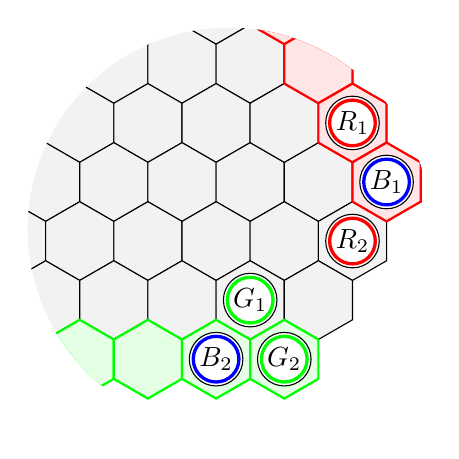
\begin{tikzpicture}
        \clip (+0.6,-0.6)  circle (2.56);
        \board
        \hex{+3}{+0}{red}{}
        \hex{+2}{+1}{red}{}
        \hex{+1}{+2}{red}{}
        \hex{+0}{+3}{red}{}
        \hex{-3}{+0}{green}{}
        \hex{-3}{+1}{green}{}
        \hex{-3}{+2}{green}{}
        \hex{-3}{+3}{green}{}
        \piece{-2}{+2}{green}{G_1}
        \piece{-3}{+3}{green}{G_2}
        \piece{+1}{+2}{red}{R_1}
        \piece{-1}{+3}{red}{R_2}
        \piece{+0}{+3}{blue}{B_1}
        \piece{-3}{+2}{blue}{B_2}
    \end{tikzpicture}
    \caption{\label{fig:exit-eg}
        In this configuration, only $R_1$ and $G_2$ have available
        \textbf{exit actions}:
        they occupy hexes marked for their colour in \Cref{fig:exits}.
        $B_1$, $B_2$ and $R_2$ also occupy hexes on edges of the board,
        but they are not on the correct edges to exit for their respective
        colours. Note that it is not possible to `jump off the board': For
        example, even though $G_1$ has an adjacent piece between it and the
        edge of the board opposite Green's starting position, $G_1$ does not
        occupy a hex marked $g$ in \Cref{fig:exits}, so it has \emph{no
        available exiting action}.
    }
\end{subfigure}
\caption{\label{fig:exit}
    These diagrams demonstrate the rules for exiting actions.
}
\end{figure}

\section*{Ending the game}

The game ends as soon as any player has taken 4 exiting actions (as
described above). That player wins the game, and the other two players
lose the game. Note that it is not enough simply to have 4 pieces `in
position' for exit actions: a turn must be taken to carry out each of
the 4 exit actions to win.

Alternatively, the game may end in a draw with no players winning the
game. A draw is declared if either of the following conditions are met:

\begin{itemize}
    \item
        One board configuration (with the same pieces occupying the same
        hexes on the same player's turn, ignoring rearrangements of
        same-coloured pieces) occurs for a fourth time since the start of
        the game.
        These repeated board configurations do not need to occur in
        succession.
    \item
        Each player has had their 256\textsuperscript{th} turn (including
        turns where the player must pass) and no winner has been declared.
\end{itemize}

\end{document}
